\usetikzlibrary{arrows.meta,calc,patterns}
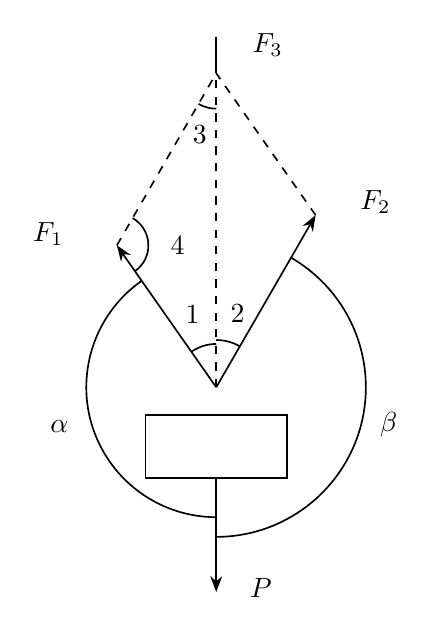
\begin{tikzpicture}[x=1cm,y=1cm,font=\normalsize,line width=.6pt,>=Stealth]
\coordinate (O) at (0,0);
\coordinate (L) at (-1.2619,1.8021);
\coordinate (R) at (1.2619,2.1856);
\coordinate (T) at (0,3.9878);
\coordinate (TE) at (0,4.45);
\coordinate (B1) at (-0.9,-1.15);
\coordinate (B2) at (0.9,-1.15);
\coordinate (B3) at (0.9,-0.35);
\coordinate (B4) at (-0.9,-0.35);
\coordinate (P0) at (0,-1.15);
\coordinate (P) at (0,-2.6);
\coordinate (ALPHA_TOP) at (-0.12,0);
\coordinate (ALPHA_BOT) at (0,-1.9);
\coordinate (BETA_TOP) at (0.12,0);
\coordinate (BETA_BOT) at (0,-2.15);
\coordinate (F1) at (-1.86,1.95);
\coordinate (F2) at (1.75,2.35);
\coordinate (F3) at (0.38,4.35);
\coordinate (PL) at (0.35,-2.55);
\coordinate (alpha) at (-1.8,-.50);
\coordinate (beta) at (2.0,-.48);
\coordinate (N1) at (-0.3,0.92);
\coordinate (N2) at (0.27,0.93);
\coordinate (N3) at (-0.21,3.21);
\coordinate (N4) at (-0.66,1.80);
\draw[dashed] (O)--(T);
\draw[dashed] (L)--(T);
\draw[dashed] (R)--(T);
\draw[->] (O)--(L);
\draw[->] (O)--(R);
\draw (T)--(TE);
\draw[->] (P0)--(P);
\draw (B4)--(B3)--(B2)--(B1)--cycle;
\draw (O) + (125:1.65) arc (125:270:1.65);
\draw (O) + (-90:1.90) arc (-90:60:1.90);
\draw (O) + (90:0.55) arc (90:125:0.55);
\draw (O) + (60:0.6) arc (60:90:0.6);
\draw (T) + (240:0.45) arc (240:270:0.45);
\draw (L) + (-55:0.40) arc (-55:60:0.40);
\node[anchor=east,inner sep=2pt] at (F1) {$F_1$};
\node[anchor=west,inner sep=2pt] at (F2) {$F_2$};
\node[anchor=west,inner sep=2pt] at (F3) {$F_3$};
\node[anchor=west,inner sep=2pt] at (PL) {$P$};
\node[anchor=east,inner sep=2pt] at (alpha) {$\alpha$};
\node[anchor=west,inner sep=2pt] at (beta) {$\beta$};
\node[anchor=center,inner sep=2pt] at (N1) {$1$};
\node[anchor=center,inner sep=2pt] at (N2) {$2$};
\node[anchor=center,inner sep=2pt] at (N3) {$3$};
\node[anchor=west,inner sep=2pt] at (N4) {$4$};
\end{tikzpicture}
